\documentclass{article}

\usepackage{amsmath, amsthm}
\usepackage{listings, xcolor}
\usepackage{graphicx}
\usepackage[pdfborder=000]{hyperref}
\usepackage{subfig}
%\usepackage{booktabs}

\title{CLab-3 Report}
\author{Jeff Yuanbo Han\quad u6617017}
\date{April 29, 2018}

\graphicspath{{figures/}}

\lstset{
	columns=fixed,
	numbers=left,
	frame=none,
	keywordstyle=\color[RGB]{40,40,255},
	numberstyle=\footnotesize\color{darkgray},
	commentstyle=\it\color[RGB]{0,96,96},
	stringstyle=\rmfamily\slshape\color[RGB]{128,0,0},
	showstringspaces=false,
	language=Matlab,
}

\newcommand*{\A}{\mathrm{A}}
\newcommand*{\sumi}{\sum_{i=1}^}
\newcommand*{\xm}{\mathbf{x}_m}
\newcommand*{\xn}{\mathbf{x}_n}
\newcommand*{\HH}{\mathbf{H}}
\theoremstyle{plain} \newtheorem{prop}{Proposition}

\begin{document}
\maketitle
\tableofcontents

\section{Face Recognition Using Eigenface}
\subsection{Preprocessing by Viola-Jones}
As we know, one of the major limitations of eigenface technique is the poor robustness to misalignment. Thus, before performing PCA, I first crop each face images into a  $200\times230$ window, which makes the face region roughly at the same position. (See \hyperref[fig-1]{Figure~1} for instance.)

\begin{figure}
	\centering
	\subfloat{
		\centering
		\fbox{
			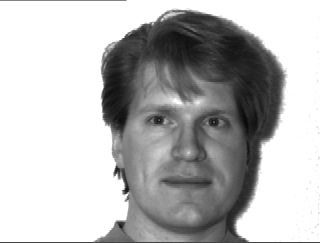
\includegraphics[width=160pt, height=121.5pt]{before_crop.png}}
	}
	\subfloat{
		\centering
		\fbox{
			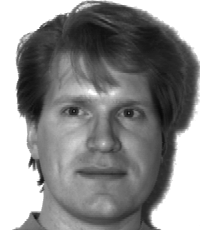
\includegraphics[width=100pt, height=115pt]{after_crop.png}}
	}
	\caption{Image before ($320\times243$) \& after ($200\times230$) preprocessing}
	\label{fig-1}
\end{figure}

This preprocessing is not done manually. Instead, I make full use of Viola-Jones Adaboost face detection. Our task is to implement face recognition using eigenface technique, which implicitly suggests that we have already known there exist a face in each image. Therefore, applying another efficient face detection method does not defeat our recognition target. A myriad of advantages are guaranteed. For example, it obviously runs much faster than a manual approach; also the alignment is expected to be more precise.

In addition, the data matrix $\Phi$, whose columns are training vectors, can be derived simultaneously during image preprocessing. Details are in the script \hyperref[code-1]{$cropImages.m$}.

\subsection{PCA}
After subtracting the mean values from $\Phi$, we are now going to implement PCA (Principle Component Analysis). This is traditionally done by computing the eigenvalues and eigenvectors of $\frac{1}{m}\Phi\Phi'$. However in this task, $\Phi$ is a $46000\times135$ matrix, and therefore $\Phi\Phi'$ is $46000\times46000$. To compute (totally $46000$) eigenvectors of such an enormous matrix is seriously time-consuming. In fact, I had waited for 2 hours on my laptop, but still got no results. On the other hand, if we swap the two matrices (i.e. $\Phi$ and $\Phi'$), we will get an only $135\times135$ $\Phi'\Phi$, which is quite easy to handle. Does it make sense to deal with $\Phi'\Phi$ rather than $\Phi\Phi'$? The answer is ``Yes''!

\begin{prop}
For any real matrix $\A$, $\A\A'$ and $\A'\A$ share the same non-zero eigenvalues.
\end{prop}
\begin{proof}
Let $\lambda$ be a non-zero eigenvalue of $\A'\A$. There must exist a corresponding eigenvector $\alpha$, such that $\A'\A\alpha = \lambda\alpha$.

Premultiply $\A$,
\begin{equation}
\label{eq-1}
\A\A'(\A\alpha) = \lambda(\A\alpha)
\end{equation}

Thus, $\lambda$ is also an eigenvalue of $\A\A'$, and $\A\alpha$ is a corresponding eigenvector.

Due to symmetry, $\A\A'$ and $\A'\A$ have common non-zero eigenvalues.
\end{proof}

Recall that when choosing $K$ (i.e. the dimension of face subspace), the criterion is
\begin{equation}
\text{Information retention} = \frac{\sumi{K}\lambda_i}{\sumi{N}\lambda_i} > Threshold
\end{equation}

In this formula, zero eigenvalues do not contribute to how much information is preserved. So we shall safely handle $\frac{1}{m}\Phi'\Phi$ instead of $\frac{1}{m}\Phi\Phi'$. After deriving eigenvalues and eigenvectors of $\frac{1}{m}\Phi'\Phi$, simply premultiply $\Phi$ to get the eigenvectors of $\frac{1}{m}\Phi\Phi'$, as suggested in \eqref{eq-1}.

Finally, for $K=5$, PCA preserves $54.50\%$ information. Top 5 eigenfaces are shown in \hyperref[fig-2]{Figure~2}. And for $K=10$, $69.84\%$ information is preserved. \hyperref[fig-3]{Figure~3} shows the top 10 eigenfaces.
\begin{figure}
\centering
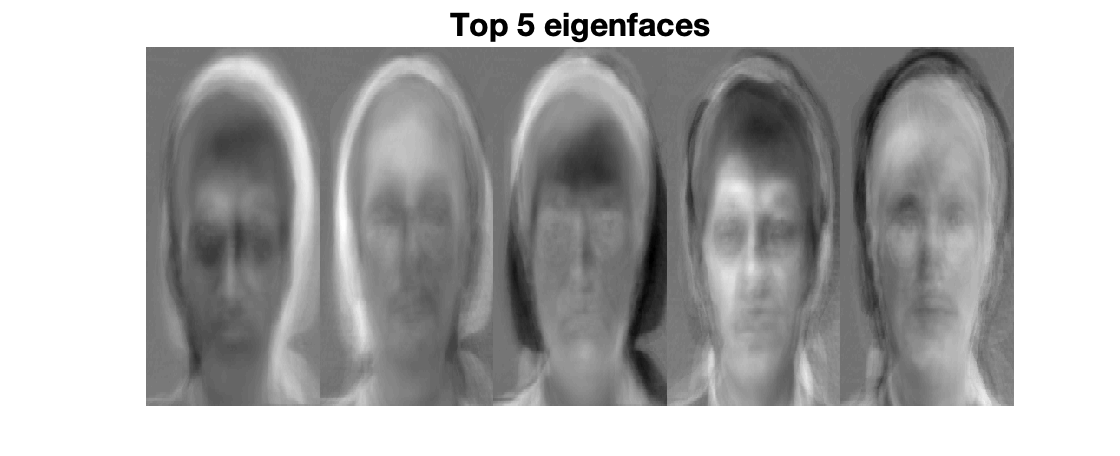
\includegraphics[width=350pt, height=80.5pt]{eigenfaces_5.png}
\caption{Top 5 eigenfaces}
\label{fig-2}
\end{figure}
\begin{figure}
	\centering
	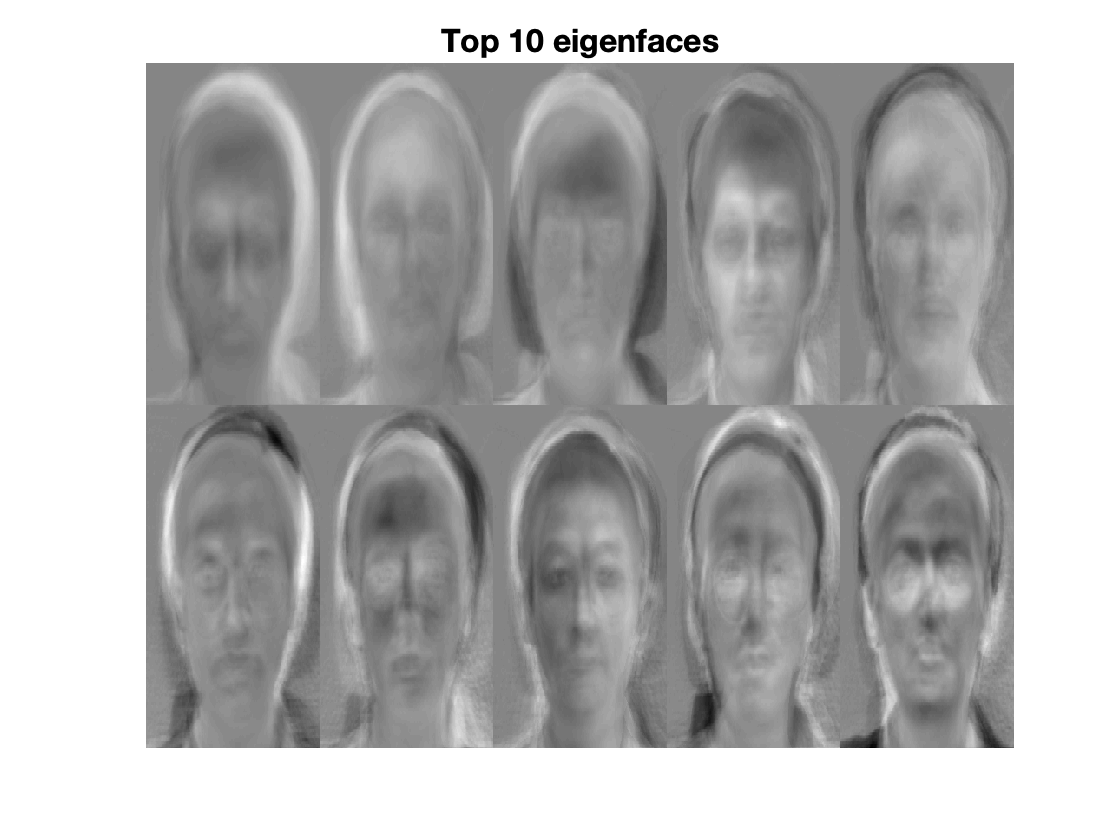
\includegraphics[width=350pt, height=161pt]{eigenfaces_10.png}
	\caption{Top 10 eigenfaces}
	\label{fig-3}
\end{figure}

\subsection{Face Recognition}
For each of the 10 test images, subtract the mean values of training data, and then project it onto the $K$-dimension face space (spanned by the top $K$ eigenfaces derived in Section~1.2). Find its nearest neighbor over all the 135 training faces.

As a result, whether to set $K=5$ or $K=10$ do not affect the final classification, although there are tinny differences when assigning nearest neighbors. (Note that each person has 9 expressions. They are different images but belong to the same person.)

The statistics of both $K=5$ and $K=10$ are displayed below. And the most 3 similar faces given by $K=5$ and $K=10$ are respectively shown in \hyperref[fig-4]{Figure~4} and \hyperref[fig-5]{Figure~5}.

\begin{verbatim}
k = 5, PCA preserves 54.50% information.
The nearest neighbor:
8     7    15    18    21    98   102   102   118   132

Classify as:
1     1     2     2     3    11    12    12    14    15

Distance in face space:
1.0e+03 *

1.4556    1.5220    0.6961    1.5110    1.8167
3.5470    2.3871    2.2000    1.3351    0.8185

k = 10, PCA preserves 69.84% information.
The nearest neighbor:
7     7    15    18    21    99   102   106   118   132

Classify as:
1     1     2     2     3    11    12    12    14    15

Distance in face space:
1.0e+03 *

2.0890    1.6177    1.7875    1.9581    2.1182
4.3596    3.1372    3.3761    1.9832    1.1773
\end{verbatim}

\begin{figure}
	\centering
	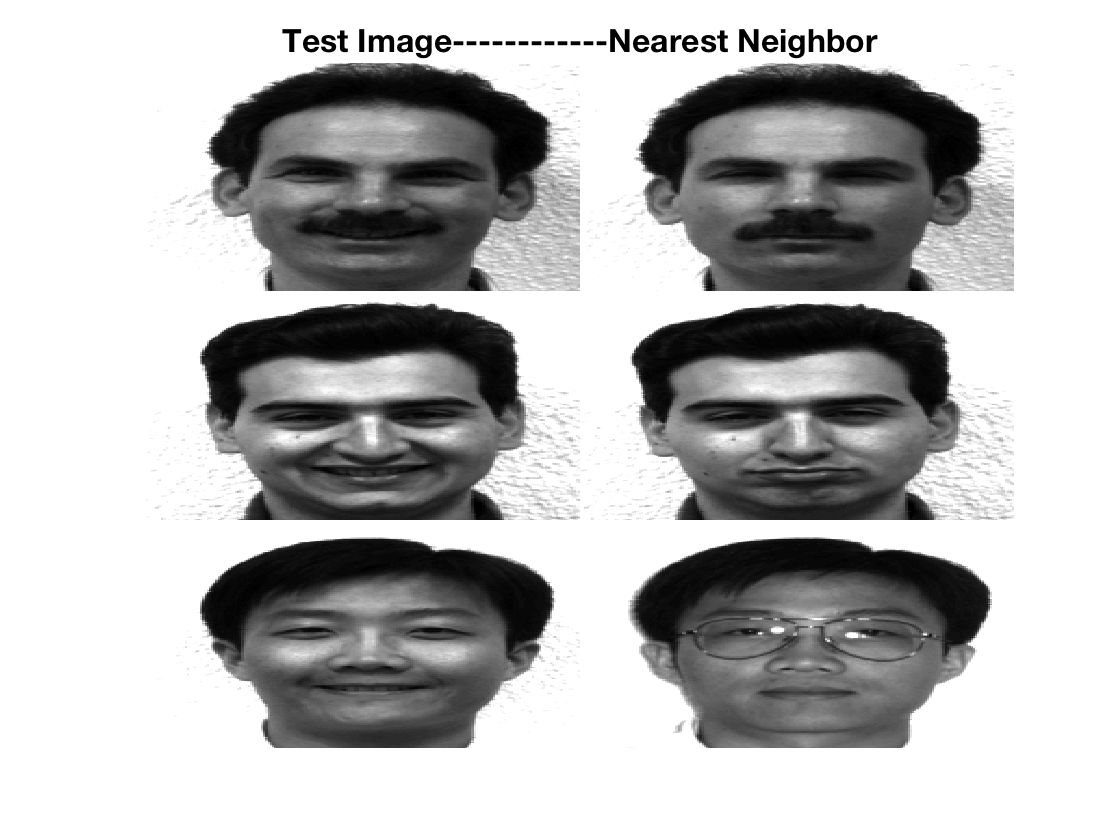
\includegraphics[width=300pt, height=345pt]{similar_faces_5.png}
	\caption{The most 3 similar faces given by $K=5$}
	\label{fig-4}
\end{figure}

\begin{figure}
	\centering
	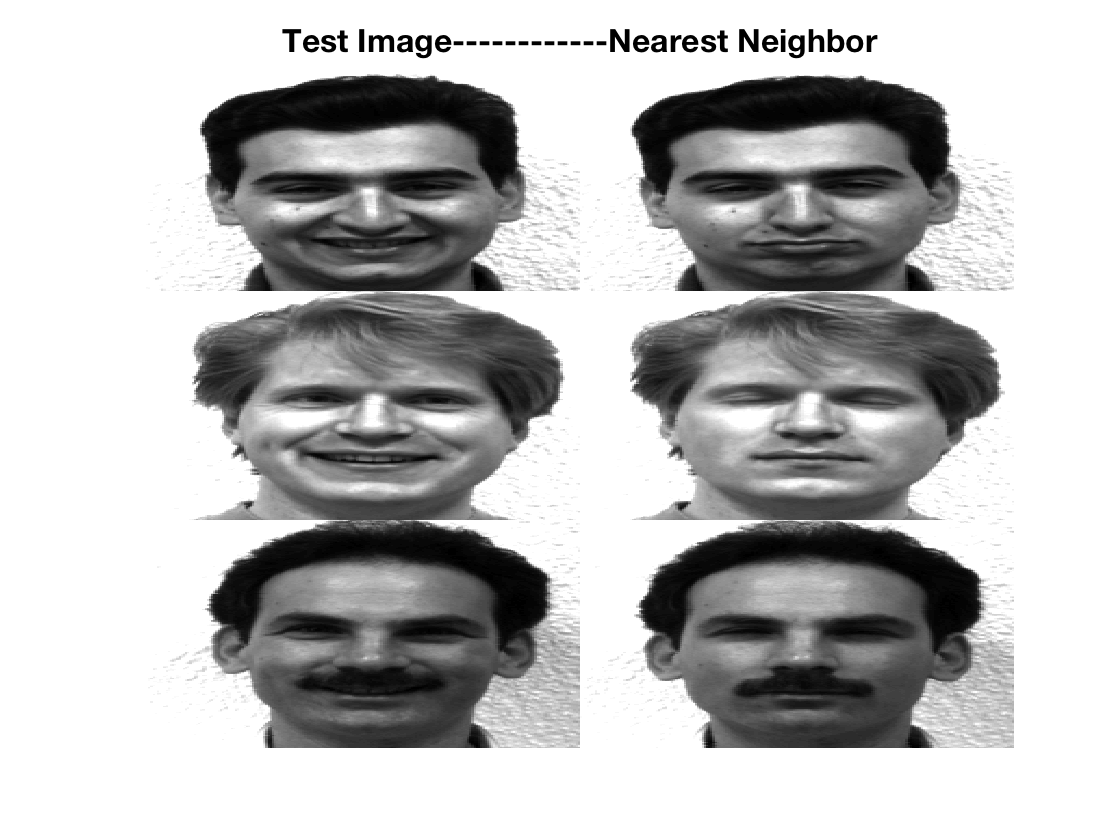
\includegraphics[width=300pt, height=345pt]{similar_faces_10.png}
	\caption{The most 3 similar faces given by $K=10$}
	\label{fig-5}
\end{figure}


\section{DLT for 2-View Homography Estimation}
\subsection{Estimation of Homography}
The 6 pairs of corresponding points I picked are shown in red in \hyperref[fig-6]{Figure~6}. And my estimation of H (i.e. the Homograpy matrix) is:
\begin{verbatim}
H =

-0.0135    0.0001    0.9950
-0.0024   -0.0058    0.0986
-0.0000    0.0000   -0.0037
\end{verbatim}

\begin{figure}
	\centering
	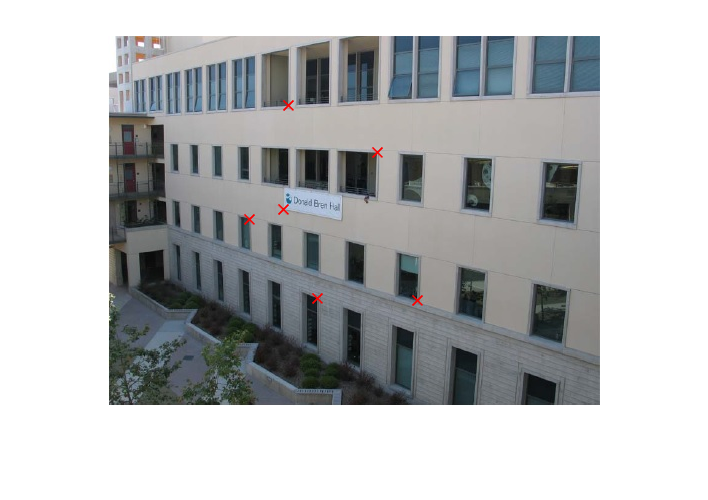
\includegraphics[scale=0.5]{Left_marked.png}
	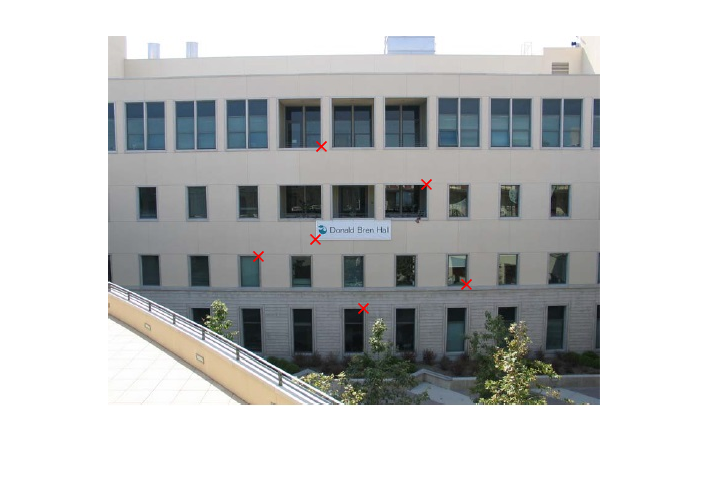
\includegraphics[scale=0.5]{Right_marked.png}
	\caption{6 corresponding (red) points for estimation}
	\label{fig-6}
\end{figure}

\subsection{Minimal Requirement for Points}
\begin{prop}
At least 4 points are required for applying DLT to estimate a 2-view Homography.
\end{prop}
\begin{proof}
Let $\xm$ and $\xn$ be a pair of corresponding points. They are supposed to satisfy:
\[
\xn = \HH\xm \Rightarrow \xn\times\HH\xm = 0
\]
Let
\begin{align*}
\xm &= (x, y, 1)^T \\
\xn &= (x', y', 1)^T \\
\HH & = \begin{pmatrix}
h_1^T \\
h_2^T \\
h_3^T
\end{pmatrix}
\end{align*}
Then
\[
\xn\times\HH\xm = \begin{pmatrix}
y'h_3^T\xm - h_2^T\xm \\
h_1^T\xm - x'h_3^T\xm \\
x'h_2^T\xm - y'h_1^T\xm
\end{pmatrix}
\]
Factorize the unknown parameters,
\[
\begin{bmatrix}
0^T & -\xm^T & y'\xm^T \\
\xm^T & 0^T & -x'\xm^T \\
-y'\xm^T & x'\xm^T & 0^T
\end{bmatrix}
\begin{pmatrix}
h_1 \\
h_2 \\
h_3
\end{pmatrix} = 0
\]

As we can see, this pair of points can provide 3 equations. However, only 2 out of them are linearly independent.

In a 2-view Homography $3\times3$ matrix, there are 8 degrees of freedom in total. Thus, we need at least 4 pairs of corresponding points to solve all the 8 parameters.
\end{proof}

\appendix
\section{MATLAB Codes}
\subsection{Face Recognition Using Eigenface}
\subsubsection{$cropImages.m$}
\label{code-1}
\begin{lstlisting}
% By Jeff Yuanbo Han (u6617017), 2018-04-24.
%% Read all the 145 face images
imgPath_train = 'yalefaces/trainingset/';
imgDir_train = dir(imgPath_train);
imgPath_test = 'yalefaces/testset/';
imgDir_test = dir(imgPath_test);

m = 135; % Total number of training images
n = 10; % Total number of test images
img = cell(m+n,1);
for i = 1:m
img{i} = imread([imgPath_train imgDir_train(i+2).name]);
end
for i = m+1:m+n
img{i} = imread([imgPath_test imgDir_test(i-m+2).name]);
end

%% Viola-Jones Face Detection
faceDetector = vision.CascadeObjectDetector; % Default: finds faces

% Window size after cropping
width = 200;
height = 230;

% Phi matrix (columns are the training vectors)
Phi = repmat(255, [width*height, m]);

for i = 1:m+n
bboxes = step(faceDetector, img{i}); % Detect the face

bboxes(1) = bboxes(1) - 30;
bboxes(2) = 10;
bboxes(3:4) = [width-1, height-1];

% Crop the image
img{i} = imcrop(img{i}, bboxes);

% Construct Phi matrix
if i <= m
[row, col] = size(img{i});
Phi(1:row*col, i) = img{i}(:);
end
end

X_bar = mean(Phi, 2);
Phi = Phi - repmat(X_bar, [1,m]);

%% Save images and data
newDir_train = 'yalefaces/trainingset_new';
mkdir(newDir_train);
newDir_test = 'yalefaces/testset_new';
mkdir(newDir_test);
for i = 1:m
imwrite(img{i}, [newDir_train '/' imgDir_train(i+2).name], 'PNG');
end
for i = m+1:m+n
imwrite(img{i}, [newDir_test '/' imgDir_test(i-m+2).name], 'PNG');
end

save train_data.mat img Phi X_bar width height

\end{lstlisting}

\subsubsection{$pca.m$}
\label{code-2}
\begin{lstlisting}
% By Jeff Yuanbo Han (u6617017), 2018-04-26.
load train_data;

%% Compute eigenvalues and eigenvectors
m = size(Phi, 2);
% Consider Phi'*Phi/m instead, for computational feasibility.
[V, D] = eig(Phi'*Phi/m);
% Derive eigenvectors of Phi*Phi'/m
V = Phi * V;
% Sort them in an ascending order
[lambda, order] = sort(diag(D),'descend');
V = V(:, order);
% Normalization
for i = 1:m
V(:,i) = V(:,i) ./ norm(V(:,i));
end

save train_data.mat lambda V -append

%% Choose k and plot eigenfaces
k = 10;
fprintf('k = %d, PCA preserves %.2f%% information.\n',...
k, 100*sum(lambda(1:k))/sum(lambda));

% Combine eigenfaces together
nTileCol = 5;
nTileRow = ceil(k/nTileCol);
Y = zeros(height*nTileRow, width*nTileCol); % to store all images
for j = 1:k
row = ceil(j/nTileCol);
col = j - nTileCol*(row-1);
Y((row-1)*height+1:row*height, (col-1)*width+1:col*width) =...
reshape(V(:,j), [height,width]);
end

figure; imagesc(Y);
colormap(gray); axis off;
title(['Top ',num2str(k),' eigenfaces'], 'FontSize', 16);

\end{lstlisting}

\subsubsection{$pcaRecog.m$}
\label{code-3}
\begin{lstlisting}
% By Jeff Yuanbo Han (u6617017), 2018-04-26.

load train_data.mat;
[pixels, m] = size(Phi); % numbers of pixels and training images
n = size(img,1) - m; % number of test images

% Vectorize test images
Phi_test = zeros(pixels, n);
for i = 1:n
Phi_test(:,i) = double(img{m+i}(:)) - X_bar;
end

%% Recognition using eigenfaces
k = 10; % First choose k

% Project onto the k-dimension subspace
Omega = V(:,1:k)' * Phi;
Omega_test = V(:,1:k)' * Phi_test;

% Find the nearest neighbor
distances = dist(Omega', Omega_test);

[difs, neighbor] = min(distances); % distances in face space
classify = ceil(neighbor/9); % number of person (each has 9 expressions)

fprintf('k = %d, PCA preserves %.2f%% information.\n',...
k, 100*sum(lambda(1:k))/sum(lambda));
fprintf('The nearest neighbor:\n'); disp(neighbor);
fprintf('Classify as:\n'); disp(classify);
fprintf('Distance in face space:\n'); disp(difs);

% Display the most three similar faces in pair
[~, index] = sort(difs);

Y = zeros(3*height, 2*width);
for j = 1:3
Y((j-1)*height+1:j*height, 1:width) = img{m+index(j)};
Y((j-1)*height+1:j*height, width+1:width*2) = img{neighbor(index(j))};
end

figure; imagesc(Y);
colormap(gray); axis off;
title('Test Image------------Nearest Neighbor', 'FontSize', 16);

\end{lstlisting}

\subsection{DLT for 2-View Homography Estimation}
\subsubsection{$DLT.m$}
\label{code-4}
\begin{lstlisting}
function [H] = DLT(u2Trans, v2Trans, uBase, vBase)
% DLT(u2Trans, v2Trans, uBase, vBase) computes the homography H,
% applying the Direct Linear Transformation.
%
% The transformation is such that
% p2 = H * p1, i.e.:
% (uBase, vBase, 1)' = H * (u2Trans, v2Trans, 1)'
%
% INPUTS:
% u2Trans, v2Trans - vectors with coordinates u and v of the transformed
%                    image point p1
% uBase, vBase - vectors with coordinates u and v of the original base
%                    image point p2
%
% OUTPUT:
% H - a 3x3 homography matrix
%
% By Jeff Yuanbo Han (u6617017), 2018-04-26.
n = max(size(u2Trans)); % number of points
A = zeros(2*n, 9);
for i = 1:n
A(2*i-1, 4:6) = -[u2Trans(i), v2Trans(i), 1];
A(2*i-1, 7:9) = vBase(i) * [u2Trans(i), v2Trans(i), 1];
A(2*i, 1:3) = [u2Trans(i), v2Trans(i), 1];
A(2*i, 7:9) = -uBase(i) * [u2Trans(i), v2Trans(i), 1];
end

[~,~,V] = svd(A);
H = reshape(V(:,end), [3,3])';
end

\end{lstlisting}

\subsubsection{$estimateH.m$}
\label{code-5}
\begin{lstlisting}
% By Jeff Yuanbo Han (u6617017), 2018-04-26.

img_L = imread('Left.jpg');
img_R = imread('Right.jpg');

n = 6;

figure; imshow(img_L);
for i = 1:n
[X_L(i), Y_L(i)] = ginput(1);
hold on;
plot(X_L(i), Y_L(i), 'rx');
end

figure; imshow(img_R);
for i = 1:n
[X_R(i), Y_R(i)] = ginput(1);
hold on;
plot(X_R(i), Y_R(i), 'rx');
end

H = DLT(X_L, Y_L, X_R, Y_R);
disp(H);

save H_estimate.mat X_L Y_L X_R Y_R H

\end{lstlisting}

\end{document}